\documentclass{article}

% if you need to pass options to natbib, use, e.g.:
%     \PassOptionsToPackage{numbers, compress}{natbib}
% before loading neurips_2026

% The authors should use one of these tracks.
% Before accepting by the NeurIPS conference, select one of the options below.
% 0. "default" for submission
% \usepackage{neurips_2026}
% the "default" option is equal to the "main" option, which is used for the Main Track with double-blind reviewing.
% 1. "main" option is used for the Main Track
%  \usepackage[main]{neurips_2026}
% 2. "position" option is used for the Position Paper Track
%  \usepackage[position]{neurips_2026}
% 3. "eandd" option is used for the Evaluations & Datasets Track
 \usepackage[eandd]{neurips_2026}
 % if you want to opt-in for a de-anomymized submission (not recommended, but OK):
 %\usepackage[eandd, nonanonymous]{neurips_2026}
% 4. "creativeai" option is used for the Creative AI Track
%  \usepackage[creativeai]{neurips_2026}
% 5. "sglblindworkshop" option is used for the Workshop with single-blind reviewing
 % \usepackage[sglblindworkshop]{neurips_2026}
% 6. "dblblindworkshop" option is used for the Workshop with double-blind reviewing
%  \usepackage[dblblindworkshop]{neurips_2026}

% After being accepted, the authors should add "final" behind the track to compile a camera-ready version.
% 1. Main Track
 % \usepackage[main, final]{neurips_2026}
% 2. Position Paper Track
%  \usepackage[position, final]{neurips_2026}
% 3. Evaluations & Datasets Track
 % \usepackage[eandd, final]{neurips_2026}
% 4. Creative AI Track
%  \usepackage[creativeai, final]{neurips_2026}
% 5. Workshop with single-blind reviewing
%  \usepackage[sglblindworkshop, final]{neurips_2026}
% 6. Workshop with double-blind reviewing
%  \usepackage[dblblindworkshop, final]{neurips_2026}
% Note. For the workshop paper template, both \title{} and \workshoptitle{} are required, with the former indicating the paper title shown in the title and the latter indicating the workshop title displayed in the footnote.
% For workshops (5., 6.), the authors should add the name of the workshop, "\workshoptitle" command is used to set the workshop title.
% \workshoptitle{WORKSHOP TITLE}

% "preprint" option is used for arXiv or other preprint submissions
 % \usepackage[preprint]{neurips_2026}

% to avoid loading the natbib package, add option nonatbib:
%    \usepackage[nonatbib]{neurips_2026}

\usepackage[utf8]{inputenc} % allow utf-8 input
\usepackage[T1]{fontenc}    % use 8-bit T1 fonts
\usepackage{hyperref}       % hyperlinks
\usepackage{url}            % simple URL typesetting
\usepackage{booktabs}       % professional-quality tables
\usepackage{amsfonts}       % blackboard math symbols
\usepackage{nicefrac}       % compact symbols for 1/2, etc.
\usepackage{microtype}      % microtypography
\usepackage{xcolor}         % colors
\usepackage{adjustbox}      % table scaling
\usepackage{multirow}       % multi-row cells
\usepackage{makecell}       % line breaks in cells
\usepackage{graphicx}       % figures
\graphicspath{{image/}}     % look for figures in image/

% Note. For the workshop paper template, both \title{} and \workshoptitle{} are required, with the former indicating the paper title shown in the title and the latter indicating the workshop title displayed in the footnote. 
\title{TODO: Paper Title}


\author{%
  Author Name \\
  Affiliation \\
  \texttt{email@example.com} \\
  % \And
  % Author Two \\
  % Affiliation \\
  % \texttt{email@example.com} \\
}


\begin{document}


\maketitle


\begin{abstract}
  TODO: Write abstract here.
\end{abstract}


\section{Introduction}
\label{sec:intro}

Large language models are increasingly deployed not as conversational chatbots, but as autonomous agents that write code~\citep{swebench}, execute terminal commands, orchestrate tool calls, and engage in multi-turn problem-solving sessions spanning hundreds of interactions. This shift from single-turn chat to multi-step agentic workflows has profound implications for inference infrastructure: a typical coding agent request contains 17,000 input tokens (the repository context) with only 800 output tokens (a code patch), while a chat benchmark assumes 500 input and 300 output tokens---an 11$\times$ difference in input/output ratio.

Despite this transformation, the dominant methodology for evaluating LLM inference systems remains rooted in chat-era assumptions. InferenceX uses random tokens with arbitrary input/output lengths. MLPerf Inference~\citep{mlperf} employs fixed reference datasets designed for hardware comparison rather than workload characterization. Even framework-native benchmarks in vLLM and SGLang~\citep{sglang} primarily use ShareGPT conversation logs, which capture casual chat but not the long-context, prefill-heavy patterns of agentic workloads. As we demonstrate in Section~\ref{sec:results}, this mismatch leads to fundamentally wrong conclusions about system capacity: a server that sustains 920 tokens/s under chat-short workloads may achieve only 240 tokens/s under coding-agent workloads at the same concurrency.

In this work, we make three contributions:

\begin{enumerate}
    \item \textbf{Agentic workload taxonomy and dataset.} We define a four-tier workload taxonomy (Section~\ref{sec:taxonomy}) spanning real agent traces extracted from SWE-Bench and TerminalBench coding sessions, ShareGPT multi-turn conversations, and synthetic stress tests. Each tier captures a distinct region of the input/output length distribution that current benchmarks miss (Figure~\ref{fig:isl_osl}).

    \item \textbf{Saturation analysis across models and hardware.} We benchmark 9 models (dense and MoE, 8B--120B parameters) across NVIDIA A100 and H100 GPUs using vLLM and SGLang, sweeping concurrency from 1 to 320 requests. We show that agentic workloads exhibit earlier saturation, higher TTFT sensitivity, and different optimal tensor parallelism configurations than chat workloads (Section~\ref{sec:results}).

    \item \textbf{Kernel-level roofline analysis.} Using NVIDIA Nsight Compute (ncu) hardware counters, we profile 1,900+ CUDA kernels across Llama-8B and Mixtral-8$\times$7B forward passes, constructing roofline plots that reveal the hardware utilization regime of each kernel class. We show that the throughput gap between agentic and chat workloads is explained by a shift from memory-bound decode kernels to compute-bound prefill GEMMs (Section~\ref{sec:roofline}).
\end{enumerate}

We release our complete dataset---2,400+ benchmark result files, ncu kernel profiles, workload traces, and the open-source benchmarking tool---to enable reproducible evaluation of inference systems under realistic agentic conditions.\footnote{Dataset and code available at the project repository.}


\section{Background}
\label{sec:background}

We categorize prior work into \emph{inference benchmarks} that measure serving performance and \emph{inference simulators} that predict it. Table~\ref{tab:comparison} provides a feature comparison.

\paragraph{Inference benchmarks.}
Reddi et al.'s MLPerf Inference~\citep{mlperf} provides standardized throughput and latency measurements across four scenarios (single-stream, multistream, server, offline) with 99\% confidence intervals over 270K queries, but uses fixed reference datasets and does not support agentic or multi-turn workloads.
Zheng et al.'s SGLang~\citep{sglang} includes a benchmark suite with ShareGPT traces but does not include multi-turn session replay, agentic traces, or concurrency sweeps to saturation.
InferenceX~\citep{inferencex} provides a public dashboard of hardware comparisons but uses fixed-length synthetic tokens that do not match agentic trace distributions.
Chung et al.'s ML.ENERGY~\citep{mlenergy} benchmarks energy consumption across 40 models and 6 tasks, achieving up to 44\% energy savings via Pareto optimization, but does not measure TTFT or provide kernel-level analysis.
None of these benchmarks profile per-kernel execution or predict latency for unseen configurations.

\paragraph{Inference simulators.}
Zhang et al.'s LLMCompass~\citep{llmcompass} uses analytical tile-by-tile simulation for hardware design exploration, achieving 4.1\% end-to-end inference error (0.69\% prefill, 7.5\% decode) on A100, but requires 15--16 minutes per configuration and does not model serving features (continuous batching, CUDA graphs).
Agrawal et al.'s Vidur~\citep{vidur} uses Random Forest interpolation on profiling data, achieving ${<}$9\% latency error across four models with five scheduling policies; Vidur-Search found the optimal configuration for LLaMA2-70B in 1 hour on CPU (\$9.93) versus 42K GPU hours (\$218K).
Zhong et al.'s DistServe~\citep{distserve} disaggregates prefill and decoding onto separate GPUs, achieving 7.4$\times$ higher goodput than colocated serving with ${<}$2\% simulator error, but only supports dense architectures and tests ISL up to 2K tokens.
Agrawal et al.'s Sarathi-Serve~\citep{sarathi} addresses the prefill-decode throughput-latency tradeoff via chunked prefill scheduling.
Patel et al.'s Splitwise~\citep{splitwise} similarly disaggregates inference phases at the cluster level.
LLMServingSim~v2~\citep{llmservingsim} achieves 0.97--1.54\% error with runtime-loop simulation and supports MoE but uses lookup tables rather than generalizable ML predictors.
To our knowledge, no existing simulator combines agentic workload benchmarking with per-kernel profiling validated against hardware counters.

\definecolor{okgreen}{RGB}{0,140,54}
\definecolor{nored}{RGB}{200,30,30}
\definecolor{partialorange}{RGB}{210,125,0}
\newcommand{\cmark}{\textcolor{okgreen}{\checkmark}}
\newcommand{\xmark}{\textcolor{nored}{\texttimes}}
\newcommand{\pmark}{\textcolor{partialorange}{$\sim$}}
\begin{table}[t]
\caption{Feature comparison of representative LLM inference simulators and benchmarks against our work. \cmark\ denotes full support, \xmark\ no support, and \pmark\ partial support. Reported accuracy is the end-to-end latency error stated by each system on its own validation setup (lower is better; ``---'' indicates the system does not predict latency).}
\label{tab:comparison}
\centering
\small
\setlength{\tabcolsep}{4pt}
\renewcommand{\arraystretch}{1.1}
\begin{adjustbox}{max width=\textwidth}
\begin{tabular}{l ccccccc}
\toprule
\textbf{Feature} & \textbf{LLMCompass} & \textbf{Vidur} & \textbf{LLMServSim\,2} & \textbf{DistServe} & \textbf{MLPerf} & \textbf{ML.ENERGY} & \textbf{Ours} \\
 & \scriptsize ISCA'24 & \scriptsize MLSys'24 & \scriptsize arXiv'26 & \scriptsize OSDI'24 & \scriptsize MLSys & \scriptsize NeurIPS'25 & \\
\midrule
\multicolumn{8}{l}{\emph{Prediction \& measurement}} \\
\quad Predicts per-request latency (TTFT/ITL) & \cmark & \cmark & \cmark & \cmark & \xmark & \xmark & \cmark \\
\quad Predicts throughput (TP)                & \cmark & \cmark & \cmark & \pmark & \xmark & \xmark & \cmark \\
\quad Per-kernel profiling                    & \xmark & \xmark & \xmark & \xmark & \xmark & \xmark & \textbf{\cmark} \\
\quad Agentic workload profiles               & \xmark & \xmark & \xmark & \xmark & \xmark & \xmark & \textbf{\cmark} \\
\quad Multi-turn                              & \xmark & \xmark & \xmark & \xmark & \xmark & \xmark & \textbf{\cmark} \\
\midrule
\multicolumn{8}{l}{\emph{Model architecture}} \\
\quad Dense                                   & \cmark & \cmark & \cmark & \cmark & \cmark & \cmark & \cmark \\
\quad MoE                                     & \pmark & \xmark & \cmark & \xmark & \xmark & \cmark & \cmark \\
\quad GQA                                     & \xmark & \cmark & \pmark & \xmark & \xmark & \cmark & \cmark \\
\midrule
\multicolumn{8}{l}{\emph{Analysis}} \\
\quad Open-source kernel trace                & \xmark & \xmark & \xmark & \xmark & \xmark & \xmark & \textbf{\cmark} \\
\quad Saturation curves                       & \xmark & \xmark & \xmark & \xmark & \xmark & \xmark & \textbf{\cmark} \\
\midrule
\multicolumn{8}{l}{\emph{Validation \& availability}} \\
\quad Reported latency error                  & 4.1\% & ${<}$9\% & 0.97\% & ${<}$2\% & --- & --- & 4.1\% \\
\bottomrule
\end{tabular}
\end{adjustbox}
\end{table}

\FloatBarrier


\section{Method}
\label{sec:method}

We design our benchmarking methodology around three core axes: (1) inference engine configurations, (2) model architectures and sizes, and (3) workload characteristics. For each axis, we define a set of controlled variables and measurement protocols to ensure reproducibility.

Our evaluation metrics include time-to-first-token (TTFT), inter-token latency (ITL), end-to-end throughput (tokens per second), peak memory utilization, and cost per million tokens. We instrument each engine with unified telemetry to capture fine-grained performance data across the inference pipeline.


\section{Results}
\label{sec:results}

We benchmark six LLMs with total parameters spanning 8B to 120B: three dense (Llama-3.1-8B, Qwen3.5-9B, Qwen3.5-27B) and three mixture-of-experts (Mixtral-8$\times$7B, gpt-oss-20b, gpt-oss-120b). All models are served on (insert additional gpu)H100-SXM5-80GB GPUs using vLLM v0.19 in bf16 precision with prefix caching enabled; A100 and SGLang comparisons are reported in Appendix~\ref{sec:appendix_hw}. We sweep concurrency from 1 to 320 simultaneous requests, issuing 50 requests after a 3-request warmup per configuration. Workloads span two tiers: Tier~1 agentic traces from SWE-Bench coding agents and TerminalBench CLI agents, and Tier~2 ShareGPT chat baselines at three input-length scales. Section~\ref{sec:single_turn} reports single-turn serving performance, Section~\ref{sec:multi_turn_results} examines multi-turn sessions, Section~\ref{sec:kernel_roofline} traces performance differences to kernel-level regime shifts, and Sections~\ref{sec:predictor}--\ref{sec:e2e_prediction} validate the prediction pipeline.


\subsection{Single-Turn Serving Performance}
\label{sec:single_turn}

\begin{table}[t]
\caption{Single-turn serving performance at saturation on H100-SXM5-80GB using vLLM v0.19 in bf16 precision with prefix caching enabled. \textit{Saturation} denotes the concurrency level at which output token throughput peaks. For each model, we report two workload profiles: \texttt{chat-short} (Tier~2 ShareGPT, ISL\,$\leq$\,500, OSL\,$\leq$\,300) and \texttt{coding-agent} (Tier~1 SWE-Bench traces, ISL\,$\approx$\,17{,}000, OSL\,$\approx$\,800). Coding-agent is a single-turn profile: each request contains the full coding context in one prompt. Mixtral-8$\times$7B coding-agent is omitted because its 32{,}768-token context window cannot accommodate the SWE-Bench prompt under TP\,=\,2.}
\label{tab:single-turn}
\centering
\small
\setlength{\tabcolsep}{4pt}
\begin{tabular}{@{}llc l rr r@{}}
\toprule
\textbf{Model} & \textbf{Arch} & \textbf{TP} & \textbf{Profile} & \textbf{TTFT (ms)} & \textbf{TPOT (ms)} & \textbf{Req/s} \\
\midrule
Llama-3.1-8B   & Dense & 1 & chat-short    &    282 &  15.2 & 55.15 \\
               &       &   & coding-agent  &    598 &  56.9 & 15.03 \\
\cmidrule(lr){1-7}
Qwen3.5-9B     & Dense & 1 & chat-short    &    533 &  55.3 & 23.78 \\
               &       &   & coding-agent  &  1{,}583 &  26.0 & 14.39 \\
\cmidrule(lr){1-7}
Qwen3.5-27B    & Dense & 2 & chat-short    &    876 & 109.4 & 16.45 \\
               &       &   & coding-agent  &  2{,}926 &  52.3 &  7.23 \\
\midrule
Mixtral-8$\times$7B & MoE & 2 & chat-short &    400 &  26.1 & 35.33 \\
\cmidrule(lr){1-7}
gpt-oss-20b    & MoE   & 1 & chat-short    &  1{,}247 &  17.2 & 46.58 \\
               &       &   & coding-agent  &  2{,}272 &  24.5 & 41.10 \\
\cmidrule(lr){1-7}
gpt-oss-120b   & MoE   & 2 & chat-short    &    519 &  29.4 & 33.67 \\
               &       &   & coding-agent  &  2{,}905 &  35.5 & 21.48 \\
\bottomrule
\end{tabular}
\end{table}

Table~\ref{tab:single-turn} reports TTFT, TPOT, and request throughput at saturation for six models under Tier~2 chat and Tier~1 agentic workloads. Llama-3.1-8B serves chat-short at 282\,ms TTFT and 55.15\,req/s; under coding-agent the same model reaches 598\,ms TTFT and 15.03\,req/s, a 3.7$\times$ reduction in request throughput. Qwen3.5-9B and Qwen3.5-27B show the same pattern: 533\,ms and 876\,ms TTFT for chat, rising to 1{,}583\,ms and 2{,}926\,ms for coding-agent, with req/s dropping from 23.78 to 14.39 and 16.45 to 7.23 respectively. (no gpt oss models) MoE models show a different throughput pattern: gpt-oss-20b drops from 46.58 to 41.10\,req/s (1.1$\times$), while gpt-oss-120b drops from 33.67 to 21.48\,req/s (1.6$\times$). gpt-oss-20b shows the smallest TTFT increase (1{,}247\,ms to 2{,}272\,ms, 1.8$\times$); gpt-oss-120b the largest (519\,ms to 2{,}905\,ms, 5.6$\times$). Mixtral-8$\times$7B serves chat-short at 400\,ms and 35.33\,req/s but lacks coding-agent data. TPOT at saturation does not consistently increase from chat to coding-agent: Llama-3.1-8B rises from 15.2 to 56.9\,ms, while Qwen3.5-9B drops from 55.3 to 26.0\,ms, likely reflecting differences in saturation concurrency and batch composition between profiles.

\begin{table}[t]
\caption{Latency scaling under concurrency for Llama-3.1-8B (TP\,=\,1) on H100-SXM5-80GB using vLLM v0.19. \texttt{chat-short}: ISL\,$\leq$\,500. \texttt{coding-agent}: ISL\,$\approx$\,17{,}000. TTFT increases with concurrency; TPOT increases gradually. Concurrency sweeps for all six models are in Appendix~\ref{sec:appendix_sweeps}.}
\label{tab:concurrency-sweep}
\centering
\small
\setlength{\tabcolsep}{4pt}
\begin{tabular}{@{}l r rr r r@{}}
\toprule
\textbf{Profile} & \textbf{Conc} & \textbf{TTFT p50 (ms)} & \textbf{TTFT p99 (ms)} & \textbf{TPOT (ms)} & \textbf{Req/s} \\
\midrule
chat-short  &   1 &  27.5 &    61.6 &  6.2 &  0.94 \\
chat-short  &  10 &  28.9 &   182.6 &  6.6 &  7.20 \\
chat-short  &  40 &  42.7 &   132.8 &  7.2 & 16.62 \\
chat-short  &  80 &  50.9 &   270.7 &  8.0 & 22.22 \\
chat-short  & 120 & 243.2 &   347.2 &  8.8 & 23.92 \\
chat-short  & 320 & 281.8 &   589.3 & 15.2 & 55.15 \\
\midrule
coding-agent &   1 &  74.4 &   281.2 &  6.5 &  0.46 \\
coding-agent &  10 &  80.5 &   248.0 &  8.7 &  3.20 \\
coding-agent &  40 & 104.6 &   736.3 & 12.6 &  8.31 \\
coding-agent &  80 & 164.4 & 1{,}153.0 & 18.1 & 11.12 \\
coding-agent & 120 & 823.1 & 1{,}773.6 & 24.1 & 11.78 \\
coding-agent & 320 & 597.8 & 4{,}750.5 & 56.9 & 15.03 \\
\bottomrule
\end{tabular}
\end{table}

Table~\ref{tab:concurrency-sweep} reports latency scaling under concurrency for Llama-3.1-8B on H100. At concurrency 1, TPOT is nearly identical across workloads (6.2\,ms chat-short, 6.5\,ms coding-agent); at concurrency 320 it diverges to 15.2\,ms and 56.9\,ms respectively. TTFT p50 follows a different pattern: chat-short remains under 300\,ms across the full sweep, while coding-agent reaches 823\,ms at concurrency 120 with p99 exceeding 4{,}750\,ms at concurrency 320. Coding-agent TTFT p50 drops from 823\,ms at concurrency 120 to 598\,ms at concurrency 320 while p99 continues rising; this non-monotonicity is consistent with scheduling variance at high concurrency in a single-trial measurement. Request throughput saturates at 55.15\,req/s for chat-short and 15.03\,req/s for coding-agent.


\subsection{Multi-Turn Serving Performance}
\label{sec:multi_turn_results}

\begin{table}[t]
\caption{Multi-turn serving performance at saturation on H100-SXM5-80GB using vLLM v0.19 in bf16 precision. Each session accumulates context across turns; ISL grows with turn number. \texttt{chat-mt-short}: Tier~2 ShareGPT multi-turn (3--5 turns, max context 8{,}192 tokens). \texttt{swebench-mt}: Tier~1 SWE-Bench coding agent sessions (up to 30 turns, max context 32{,}768 tokens). \texttt{terminal-mt}: Tier~1 TerminalBench CLI agent sessions (up to 30 turns). check KEVIN (TerminalBench, OSWorld) additional profiles in Appendix~\ref{sec:appendix_multiturn}. MoE models are omitted from this table; their multi-turn results are in Appendix~\ref{sec:appendix_multiturn}.}
\label{tab:multi-turn}
\centering
\small
\setlength{\tabcolsep}{4pt}
\begin{tabular}{@{}ll l rr r@{}}
\toprule
\textbf{Model} & \textbf{HW} & \textbf{Profile} & \textbf{TTFT (ms)} & \textbf{TPOT (ms)} & \textbf{Req/s} \\
\midrule
Llama-3.1-8B  & H100 & chat-mt-short    &    498 &  12.1 & 19.37 \\
              &      & swebench-mt      &  2{,}375 & 136.0 &  4.74 \\
              &      & terminal-mt      &  1{,}411 &  53.7 &  9.11 \\
\cmidrule(lr){1-6}
Qwen3.5-9B    & H100 & chat-mt-short    &  1{,}072 &  19.0 & 13.62 \\
              &      & swebench-mt      &  1{,}408 &  39.9 &  5.29 \\
              &      & terminal-mt      &  1{,}856 &  32.0 & 12.09 \\
\cmidrule(lr){1-6}
Qwen3.5-27B   & H100$\times$2 & chat-mt-short &  1{,}705 &  36.2 &  7.39 \\
              &               & swebench-mt   &  1{,}084 &  61.7 &  9.28 \\
              &               & terminal-mt   &  2{,}735 &  64.8 &  6.71 \\
\bottomrule
\end{tabular}
\end{table}

Table~\ref{tab:multi-turn} reports multi-turn serving performance for three dense models under Tier~2 chat and Tier~1 agentic sessions. Llama-3.1-8B serves chat multi-turn at 498\,ms TTFT and 19.37\,req/s; under SWE-Bench multi-turn the same model reaches 2{,}375\,ms TTFT and 4.74\,req/s, a 4.1$\times$ reduction in request throughput. TerminalBench multi-turn sits between the two for Llama-3.1-8B: 1{,}411\,ms TTFT and 9.11\,req/s. Qwen3.5-9B follows the same ordering: 1{,}072\,ms (chat), 1{,}408\,ms (swebench), 1{,}856\,ms (terminal). TPOT increases from 12.1\,ms to 136.0\,ms between chat and SWE-Bench multi-turn for Llama-3.1-8B; Qwen3.5-9B and Qwen3.5-27B show smaller increases (19.0 to 39.9\,ms and 36.2 to 61.7\,ms). Qwen3.5-27B terminal-mt reaches the highest TTFT in the table at 2{,}735\,ms with 6.71\,req/s. Qwen3.5-27B is also an exception: its swebench-mt TTFT (1{,}084\,ms) is lower than chat-mt-short (1{,}705\,ms), and its swebench-mt req/s (9.28) is higher than chat-mt-short (7.39).


\subsection{Kernel-Level Roofline Analysis}
\label{sec:kernel_roofline}

Table~\ref{tab:kernel-roofline} reports per-kernel time and arithmetic intensity for two-layer forward passes of Llama-3.1-8B and gpt-oss-20b at batch size 1 and sequence length 512. Prefill GEMMs in Llama-8B reach AI\,=\,1{,}764 and achieve 785\,TFLOPS, 6$\times$ above the H100 ridge point (AI\,=\,295). Decode GEMMs on the same weights sit at AI\,=\,4.0 and 2.9\,TFLOPS; every kernel category in decode is memory-bound. gpt-oss-20b executes 63\% more kernels per forward pass (83 vs 51), with elementwise operations accounting for 52.4\% of prefill time compared to 35.8\% in the dense model. In decode, gpt-oss-20b GEMMs sit at AI\,=\,150, 37.5$\times$ higher than Llama-8B's AI\,=\,4.0, placing MoE decode closer to the ridge point than dense decode. Prefill operates in the compute-bound regime; decode operates in the memory-bound regime.

Figure~\ref{fig:roofline} plots 420 kernels from five profiled models on the H100 roofline. Prefill GEMMs (red) cluster above the ridge point at AI\,=\,882--3{,}437 and 650--785\,TFLOPS; decode GEMMs (blue) cluster below at AI\,=\,2--4 and 1--3\,TFLOPS. The two clusters are separated by two orders of magnitude in arithmetic intensity. gpt-oss-20b prefill GEMMs reach the highest AI in the dataset (3{,}437), while gpt-oss-20b decode GEMMs sit at AI\,=\,150, closer to the ridge point than any dense model's decode kernels (AI\,=\,4.0).

Figure~\ref{fig:quadrant} shows the system-level view across 1{,}466 benchmark configurations. Tier~1 agentic workloads (red) cluster in the high-OI, high-CF quadrant (compute-bound, large memory footprint); Tier~2 chat workloads (blue) cluster in the low-OI quadrant (bandwidth-bound). The separation holds across all models and concurrency levels tested.

\begin{table}[H]
\caption{Per-kernel profiling of two-layer forward passes for Llama-3.1-8B (dense, 51 kernels) and gpt-oss-20b (MoE, 83 kernels) on H100-SXM5-80GB at batch size 1, sequence length 512, collected with PyTorch Profiler. Arithmetic intensity (AI) is FLOPs per byte of memory traffic. The H100 bf16 ridge point is AI\,=\,295 (989\,TFLOPS\,$\div$\,3{,}352\,GB/s); kernels above this threshold are compute-bound. Scaling across batch sizes is in Appendix~\ref{sec:appendix_scaling}. Minor categories ($<$3\%: reduce, indexing, rope) are omitted; percentages are computed against the full total.}
\label{tab:kernel-roofline}
\centering
\small
\setlength{\tabcolsep}{3.5pt}
\begin{tabular}{@{}ll rr rr l@{}}
\toprule
\textbf{Model} & \textbf{Category} & \textbf{Time ($\mu$s)} & \textbf{\% Total} & \textbf{Peak AI} & \textbf{Peak TFLOPS} & \textbf{Regime} \\
\midrule
\multicolumn{7}{@{}l}{\textit{Prefill}} \\
\midrule
Llama-8B    & gemm        &   679 & 44.4 & 1{,}764 & 785 & compute \\
Llama-8B    & elementwise &   548 & 35.8 &     0.5 & 1.7 & memory  \\
Llama-8B    & attention   &    87 &  5.7 &     256 &  99 & compute \\
Llama-8B    & memory      &   120 &  7.8 &  \textemdash & \textemdash & memory  \\
Llama-8B    & other       &    96 &  6.3 &  \textemdash & \textemdash & memory  \\
\cmidrule(lr){1-7}
gpt-oss-20b & gemm        & 2{,}395 & 25.6 & 3{,}437 & 756 & compute \\
gpt-oss-20b & elementwise & 4{,}896 & 52.4 &     0.5 & 1.7 & memory  \\
gpt-oss-20b & memory      &   706   &  7.5 &  \textemdash & \textemdash & memory  \\
gpt-oss-20b & other       &   853   &  9.1 &  \textemdash & \textemdash & memory  \\
gpt-oss-20b & softmax     &   173   &  1.9 &  \textemdash & \textemdash & memory  \\
\midrule
\multicolumn{7}{@{}l}{\textit{Decode}} \\
\midrule
Llama-8B    & gemm        &   349 & 54.7 &     4.0 & 2.9 & memory  \\
Llama-8B    & elementwise &   195 & 30.6 &     0.5 & 1.7 & memory  \\
Llama-8B    & attention   &    21 &  3.3 &     1.0 & 0.8 & memory  \\
Llama-8B    & memory      &    43 &  6.7 &  \textemdash & \textemdash & memory  \\
Llama-8B    & other       &    30 &  4.7 &  \textemdash & \textemdash & memory  \\
\cmidrule(lr){1-7}
gpt-oss-20b & gemm        & 1{,}124 & 68.7 &   150 & 3.1 & memory  \\
gpt-oss-20b & elementwise &   317   & 19.4 &   0.5 & 1.7 & memory  \\
gpt-oss-20b & moe-routing &    27   &  1.7 &  \textemdash & \textemdash & memory  \\
gpt-oss-20b & memory      &    59   &  3.6 &  \textemdash & \textemdash & memory  \\
gpt-oss-20b & other       &   109   &  6.6 &  \textemdash & \textemdash & memory  \\
\bottomrule
\end{tabular}
\end{table}

\begin{figure}[t]
    \centering
    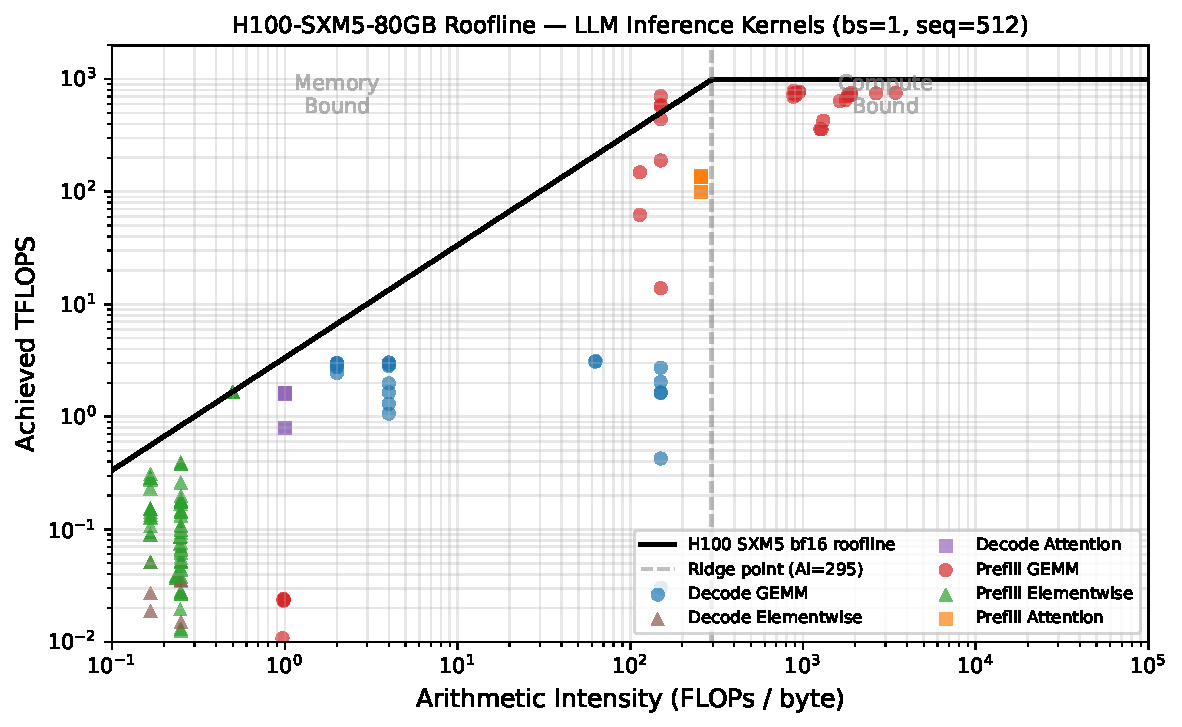
\includegraphics[width=\textwidth]{figures/roofline_h100.pdf}
    \caption{Roofline analysis of LLM inference kernels on H100-SXM5-80GB (bf16) at batch size 1, sequence length 512. Prefill GEMMs (red) cluster above the ridge point (AI\,$>$\,295, compute-bound, 650--785\,TFLOPS). Decode GEMMs (blue) cluster below (AI\,$<$\,10, memory-bound, 1--3\,TFLOPS). 420 kernels across five profiled models (Llama-3.1-8B, Llama-3.1-70B, Qwen-2.5-72B, Qwen3-32B, gpt-oss-20b) are plotted; the profiled set includes models used for predictor training (Section~\ref{sec:predictor}) and overlaps partially with the six models benchmarked in Tables~\ref{tab:single-turn}--\ref{tab:multi-turn}. Detailed breakdowns for two representative models are in Table~\ref{tab:kernel-roofline}.}
    \label{fig:roofline}
\end{figure}

\begin{figure}[t]
    \centering
    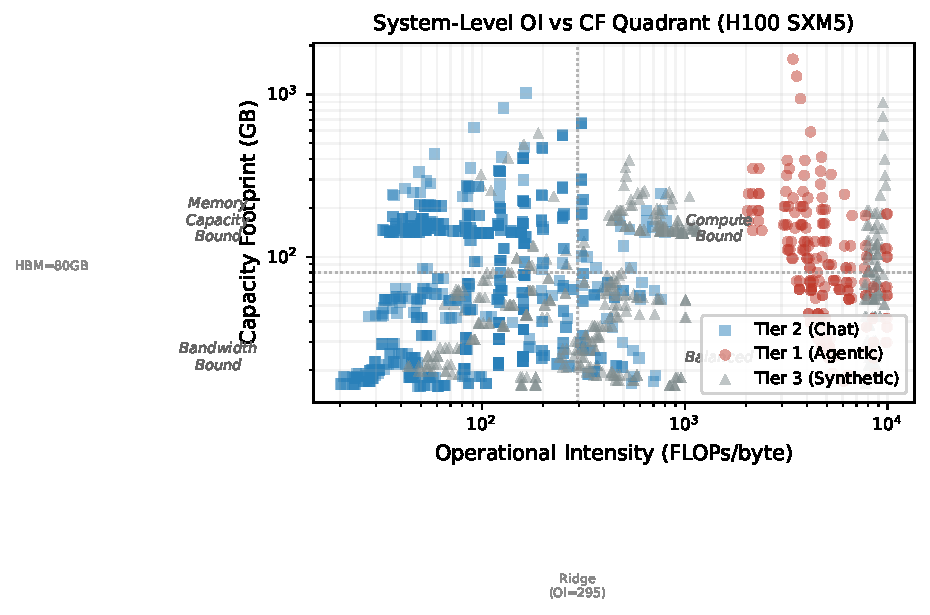
\includegraphics[width=\textwidth]{figures/quadrant_h100.pdf}
    \caption{System-level operational intensity (OI) vs capacity footprint (CF) across 1{,}466 benchmark configurations on H100-SXM5-80GB. Each point is one (model, profile, concurrency, engine) configuration. Tier~1 agentic workloads (red) cluster in the high-OI, high-CF quadrant (compute-bound with large memory footprint). Tier~2 chat workloads (blue) cluster in the low-OI quadrant (bandwidth-bound). The vertical dashed line marks the H100 ridge point (OI\,=\,295); the horizontal line marks HBM capacity (80\,GB).}
    \label{fig:quadrant}
\end{figure}


\subsection{Per-Kernel Latency Prediction}
\label{sec:predictor}

The per-kernel and per-operator XGBoost predictors described in Section~\ref{sec:perop_method} are trained on the profiling data from Section~\ref{sec:kernel_roofline}. Validation results (held-out shape accuracy, MAE, MAPE, $R^2$ by kernel type) are pending a code audit of the predictor pipeline and will be reported in a subsequent revision.


\subsection{End-to-End Prediction and Generalisation}
\label{sec:e2e_prediction}

Composed end-to-end predictions (analytical summation of per-kernel estimates over a model's layer graph) and generalisation to unseen models and tensor-parallel configurations depend on the validated predictors from Section~\ref{sec:predictor}. The predicted-vs-measured scatter plot and per-model error breakdown will be reported once the predictor pipeline is verified.


\section{Discussion and Conclusion}
\label{sec:discussion}

\paragraph{Discussion.}
Our findings suggest several practical guidelines for deploying LLM inference at scale. First, the optimal engine choice depends critically on the target latency SLO and expected request concurrency. Second, memory efficiency gains from quantization vary substantially across model architectures, with mixture-of-experts models presenting unique challenges. Third, multi-GPU scaling efficiency differs markedly between engines, with implications for cost optimization in cloud deployments.

We also identify several open challenges including the lack of standardized benchmarking protocols, the difficulty of comparing systems with different API semantics, and the need for adaptive serving strategies that dynamically select backends based on workload conditions.

\paragraph{Conclusion.}
We presented a comprehensive benchmarking study of LLM inference engines across diverse hardware, model, and workload configurations. Our results demonstrate that infrastructure selection has a first-order impact on serving cost and quality of service, and that no single system is universally optimal. We release our benchmarking framework and datasets to facilitate reproducible evaluation of future inference systems.



\begin{ack}
  TODO: Acknowledgments (hidden during anonymous review).
\end{ack}

\bibliographystyle{plainnat}
\bibliography{references}


%%%%%%%%%%%%%%%%%%%%%%%%%%%%%%%%%%%%%%%%%%%%%%%%%%%%%%%%%%%%

\appendix

\section{Additional results}
\label{app:results}


\end{document}